\noindent\textbf{UT-Interaction Dataset.} For a comparison with the state-of-art, we implement our approach on UT-Interaction dataset initially used in \cite{Ryoo:group} and recently again in \cite{Amer:group}. The dataset consists of 20 one-minute videos of continuous executions of 6 classes of two-person interactions: shaking-hands, pointing, hugging, pushing, kicking, and punching. Each video contains at least one instance of every interaction class, where distinct activities may occur at the same time. 10 videos are taken on a parking lot and the other 10 videos are captured in a natural setting by a moving camera. As the UT-Interaction dataset presents simultaneous performance of several activities, activities that may begin and end at arbitrary times, and the presence of people who are not involved in the activity, etc., it is well fitted into the scenario considered here. We follow exactly the same setup as in \cite{Ryoo:group,Amer:group}: 20\% of all available manual segmentations, each occupied by a unique activity instance, are used as `database exemplars' for training. The remaining full (unsegmented) sequences are used for testing. In training, a 4-level pyramid is set up at each ground-truth time interval, and a temporal unit is set at half length of the bottom-level cell. A 32-dimensional histogram of the spatio-temporal features developed by \cite{Dollar:STIP} in each unit and each bounding box is calculated first against a 500-word vocabulary from K-means clustering and then by PCA, and serves as the individual activity descriptor. Another 32-dimensional histogram of the optical flow computed from OpenCV in each unit and each box is calculated against 8 directions and 4 magnitudes, and the difference between the two histograms (relative motion) serves as the contextual descriptor between the two humans. In testing, we employ the human detector \cite{Pedro:detect}, and associate the detected boxes across frames to form continuous tracks of humans. 

\begin{table}[ht]
\centering \caption{Classification accuracies and false positive (FP) rates for the proposed method and the baselines on UT-Interaction dataset.}
\footnotesize{
\begin{tabular}{|c||c|c|}
\hline   & Accuracy (\cite{Ryoo:group}, \cite{Amer:group}, ours) & FP Rate (\cite{Ryoo:group}, \cite{Amer:group}, ours) \\
\hline Hug &  (0.875, 0.904, \underline{1.00}) & (0.075, 0.055, \underline{0.00}) \\
\hline Kick &  (0.750, 0.775, \underline{0.875})  & (0.138, 0.108, \underline{0.063})\\
\hline Point & (0.625, 0.663,  \underline{0.750}) & (\underline{0.025}, \underline{0.025}, 0.088)\\
\hline Punch & (0.500, 0.632, \underline{0.750})  & (0.201, 0.154,  \underline{0.138})\\
\hline Push & (0.750, \underline{0.782} , 0.750)  & (0.125, \underline{0.101},  0.138)\\
\hline Shake Hands &  (0.750, 0.789, \underline{1.00}) & (0.088, 0.060, \underline{0.00}) \\
\hline\hline Average &  (0.708, 0.758, \underline{0.854})  & (0.108, 0.083,  \underline{0.071})\\
\hline 
\end{tabular}
}
\label{UTaccuFP}
\end{table}


The first interesting investigation is again about the effectiveness of combining both individual descriptor and contextual descriptor, as well as metric learning for group dissimilarity function. We implement our approach with either but not both descriptor, and without learning the dissimilarity. The performance comparison is show in Table ~\ref{UTaccuFPdegrade}, which again proves the merit of the combined descriptors and learning optimal metrics between descriptors. It is interesting to see the contextual descriptor plays a more crucial role for this dataset: A significant performance drop arises when we only consider individual action descriptors. The next comparison is against the state-of-art methods \cite{Ryoo:group,Amer:group}. The recognition accuracies and false-alarm rates are shown in Table ~\ref{UTaccuFP}. In this evaluation, we only allow one database exemplar to produce a single response in an input, and claim a true positive only when both the class-label and the identified participants are simultaneously correct, otherwise a false positive is claimed for the exemplar class. We achieve improved accuracy and competitive false positive rate against the baselines. In the third evaluation, we specifically look into the temporal localization and participant identification performance. For temporal localization, we follow exactly the same criterion as in \cite{Amer:group}, requiring a true-positive to achieve both correct classification and a $>50\%$ ratio of the intersection to the union of the estimated interval and ground-truth. we achieve a slightly smaller area under ROC curve than the two baselines, as shown in Table ~\ref{UTarea}. Note that the temporal boundary is essentially ambiguous for these consecutively executed activities. For participant identification, we enforce an even stricter criterion to require $100\%$ correct identification (in contrast to $50\%$ in \cite{Amer:group}) for a true positive, and we outperform \cite{Amer:group}. Note that \cite{Ryoo:group} does not apply human detection and tracking and \cite{Amer:group} does not explicitly operate on the detected bounding boxes. Therefore, our performance should be regarded as an overall effect from both human detection/tracking and our group matching framework.

\begin{table}[ht]
\centering \caption{Area under ROC curve for the proposed method and the baselines on UT-Interaction dataset.}
\footnotesize{
\begin{tabular}{|c|c|c|c|}
\hline   & \cite{Ryoo:group} &  \cite{Amer:group}  &   ours \\
\hline Temporal Localization &  0.91 & \underline{0.94} &  0.89\\
\hline Participants Identification &  N/A & 0.87 &  \underline{0.93}   \\
\hline 
\end{tabular}
}
\label{UTarea}
\end{table}

\begin{table}[ht]
\centering \caption{Classification accuracies and false positive (FP) rates comparison on UT-Interaction dataset for evaluating the effectiveness of different components of the proposed approach: Individual and/or contextual descriptors, with or without metric learning (ML).}
\footnotesize{
\begin{tabular}{|c|c|c|c|}
\hline   & Individual only & Contextual only & Both \\
\hline Accur. w. ML & 0.688 & 0.813 & 0.854  \\
\hline Accur. w/o ML & 0.647 & 0.750 & 0.771    \\
\hline FP Rate w. ML &  0.125 & 0.096 & 0.071  \\
\hline FP Rate w/o ML & 0.163 & 0.113 & 0.083\\
\hline 
\end{tabular}
}
\label{UTaccuFPdegrade}
\end{table}



\vspace{0.05in}

\noindent\textbf{Caltech Resident-Intruder Mouse Dataset.} We also tested the approach on Caltech Resident-Intruder Mouse Dataset \cite{CRIM13}, which contains long video sequences recording pair-wise interactions between two mice. Behaviors are categorized into 12 different mutually exclusive action types, plus an `other' category indicating no behavior of interest is occurring. A video typically lasts around 10 minutes at 25fps with a resolution of 640x480 pixels. Every video frame is labeled with one of the thirteen ground-truth categories, resulting in a segmentation of the videos
into action intervals. For more details please refer to \cite{CRIM13}. Note that in all videos are pair-wise interactions, and our experiment on this dataset is not meant to distinguish the participants, but to demonstrate that our approach can be directly used for a traditional task of temporal segmentation and classification without any changes.

We exactly follow the training/testing partitions provided by the dataset. We extract the spatio-temporal interest points (STIP) based appearance features and compute trajectory-based features from the tracks provided with the dataset as \cite{CRIM13} does (See \cite{CRIM13} for details). Differently from \cite{CRIM13}, we only compute STIP based features inside the bounding boxes enclosing the mice. The trajectory-based features consists of those describing the motion of each individual mouse and those describing the relative motion between two mice. We denote the former as T\_ind and the latter as T\_pair. Again we use a 4-level temporal pyramid, in which the STIP based appearance features are computed as \cite{CRIM13} does and the trajectory based features are also transformed into histograms against 64 codewords. 

Three combinations of features were attempted in \cite{CRIM13}: Trajectory only, STIP only, and using both. For the case trajectory only, our approach has two possible working modes: Using all trajectory-based features as individual descriptors (denoted as Trajectory\_1), or using T\_ind as individual descriptors and using T\_pair as contextual descriptors (denoted as Trajectory\_2). In the case of STIP only, all features are used as individual descriptors, and in the case of using both, STIP features and trajectory-based features serve as individual descriptor and contextual descriptors respectively. To classify a segment responded by one or more exemplars, we simply give it the label of the top-ranked exemplar. We follow the same error metric as \cite{CRIM13}, the frame-wise accuracy, and report the results in Table \ref{CRIMAccu}, where it is evident that motion trajectory is much more discriminative than local STIP based features given little articulation in a constrained environment. The competing performance by approach is achieved by splitting the motion into individual ones and contextual ones and learning separate metrics for them (Trajectory\_2). In other cases, multi-level adaboost based approach exhibits superiority on frame-wise classifications (as in \cite{CRIM13}).


\begin{table}[ht]
\centering \caption{Accuracies for the proposed method and the baselines on Caltech Resident-Intruder Mouse Dataset. (\%)}
\footnotesize{
\begin{tabular}{|c||c|c|c|c|}
\hline   & Trajectory\_1  & Trajectory\_2 & STIP & Both \\
\hline \cite{CRIM13} w/o. context & 52.3  & 52.3 & 29.3 & 53.1\\
\hline \cite{CRIM13} w. context &  \underline{58.3} & 58.3 & \underline{43.0} & 61.2\\
\hline Ours w/o. ML &  45.6 & 49.4 & 18.8 & 50.9 \\
\hline Ours w. ML & 54.5 & \underline{66.0} & 31.7 & \underline{62.9}\\
\hline 
\end{tabular}
}
\label{CRIMAccu}
\end{table}

It is observed in \cite{CRIM13} that accuracy varies with the length of the interaction and with the length of window within which the local feature is computed. To investigate the performance of our approach on different lengths of the interaction as compared to \cite{CRIM13}, we implemented the approach in \cite{CRIM13} using trajectory-based features and one-level auto-context classifier. As shown by the result in Figure \ref{frame_no}, our approach is particularly better at localizing longer interactions though \cite{CRIM13} demonstrates its advantage under a shorter feature window on shorter interactions. 

\begin{figure}[t]
\begin{center}
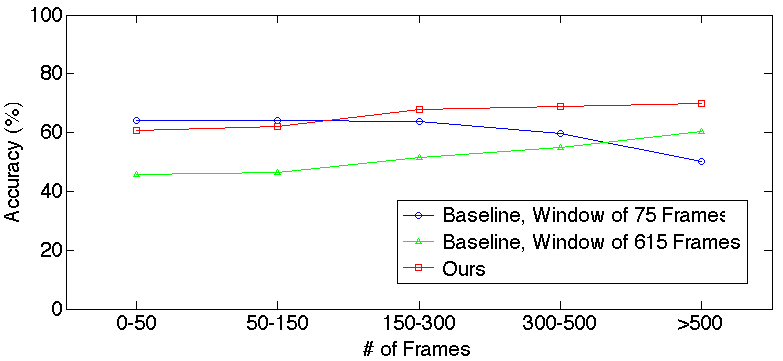
\includegraphics[scale=0.25]{frame_no.png}
\end{center}
\caption{Accuracy comparison for varying length of interactions between \cite{CRIM13} and our approach.}
\label{frame_no}
\end{figure}

\vspace{0.05in}

\noindent\textbf{Conclusion.} We have proposed an approach to find small-group social interactions in space and time among a larger group of people. We achieve simultaneous participant identification, temporal localization, and classification. These functionalities are enabled and optimized by learning the best ensemble (dis)similarities from data. Our approach is flexible and generic to various of applications provided that an individual behavior descriptor and a contextual behavior descriptor are properly defined and computed. On the other hand, a further improvement of the overall performance will also rely on the robustness and discrimination of these descriptors, especially when videos are of limited quality such as the classroom videos we use. 
